\chapter{Grundlagen}\label{pre}

Wir werden uns in dieser Arbeit hauptsächlich mit einfachen planeren Graphen beschäftigen, also solchen die keine Mehrfachkanten und Schleifen besitzen und für die kreuzungsfreie Zeichnungen, beziehungsweise Einbettungen, in der Ebene existieren. Sei $G = (V,E)$ ein Graph bestehend aus der Menge der Knoten $V$ und Kanten $E \subseteq ( \,V \times V ) \,$. Eine Kante $(u,v)$ verbindet die beiden Knoten $u$ und $v$. Ein Pfad von $u$ nach $v$ ist eine Folge von Kanten, die $u$ und $v$ verbindet. Mit dem Grad $deg(v)$ eines Knoten meinen wir die Anzahl der adjazenten Kanten.\ 

Einen planaren Graphen zusammen mit einer möglichen kreuzungsfreien Einbettung in der Ebene bezeichnen wir als \textit{planen Graphen}. Für einen planen Graphen können wir, zusätzlich zu den Knoten und Kanten, auch die Menge der Gebiete (engl. faces) $F$ betrachten, die durch die Kanten und Knoten begrenzten Regionen in der Ebene, wobei wird das unbeschränkte als das \textit{äussere} Gebiet bezeichnen. Für die weiteren Betrachtungen macht es oft Sinn drei Knoten $\{a_1,a_2,a_3\}$ die das äusseren Gebiet berühren gesondert zu betrachten. Wir nennen sie die \textit{Aufhängungen} von $G$ und bezeichnen $G$ als \textit{aufgehängten} Graphen.\

Planare Graphen haben, durch die Existenz kreuzungsfreier Einbettungen, in gewissem Sinne besonders schöne Zeichnungen und so ist einer der Fragen mit der sich schon viele Mathematiker auseinander gesetzt haben und auf die wir auch in dieser Arbeit eingehen wollen: \textit{"How to draw a Graph?"}\cite{tutte63}\\

Wir werden bei Einbettungen mit wenigen Einschränkungen beginnen. Bei einer topologischen Zeichnung eines planaren Graphen werden die Kanten als Kurven dargestellt die sich nur in den Knoten treffen. In den Fünfzigern wurde unter anderem von István Fáry gezeigt, dass für jeden planaren Graphen und für jede Wahl eines äusseren Gebietes eine geradlinige und kreuzungsfreie Einbettung existiert \cite{fary48}.

\begin{definition}[intern zusammenhängend]\label{int_3_con}
Ein Graph $G$ ist zusammenhängend falls für alle Knoten $u,v$ ein Pfad von $u$ nach $v$ exisitert. $G$ ist \textit{k-zusammenhängend}, falls er nach der Entfernung von $k-1$ beliebigen Knoten weiterhin zusammanhängend ist.\\
Sei $G$ plan mit den Aufhängungen $\{a_1,a_2,a_3\}$, weiter sei $a_\infty$ ein zusätzlicher Knoten eingefügt im äusseren Gebiet. Dann ist $G$ \textit{intern k-zusammenhängend}, falls $G=(V,E\cup \{(a_1,a_\infty),(a_2,a_\infty),(a_3,a_\infty)\})$ k-zusammenhängend ist. 
\end{definition}

In den Siebzigern betrachtete William Thomas Tutte die Unterklasse der 3-zusam-men hängenden planaren Graphen und zeigte, dass für diese nicht nur geradlinige, sondern sogar \textit{konvexe} Zeichnungen existieren, bei denen alle Gebiete, inklusive dem Äusseren, konvexe Polygone umranden \cite{tutte63}.

\begin{figure}
	\centering
  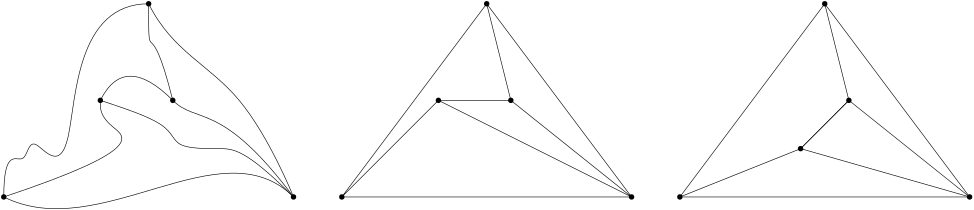
\includegraphics[width=0.9\textwidth]{topo_straight_convex.png}
	\caption{Planarer Graph mit einer topologischen, einer geradlinigen und einer konvexen Zeichnung.}
	\label{topo_straight_convex}
\end{figure}

\section{Geradlinige Dreiecks Darstellungen (SLTRs)}

Ausgehend von der konvexen Darstellung nach Tutte, kann man sich die Frage stellen unter welchen Vorraussetzungen wir einen planaren Graphen so zeichnen können, dass alle Gebiete, inklusive dem Äusseren Dreiecken umranden. Bei der Formalisierung dieser Darstellung und ersten Feststellungen halten wir uns an Nieke Aerts und Stefan Felsner \cite{af13}.

\begin{definition}[SLTR]\label{defsltr}
Eine Zeichnung eines planen Graphen $G$ wird Gradlinige Dreiecks Darstellung, im weiteren kurz \textit{SLTR} (für die englische Bezeichnung Staight Line Triangle Representation), genannt falls gilt:
\begin{itemize}
\item[S1] Alle Kanten Segmente von Geraden
\item[S2] Alle Gebiete, inklusive dem äusseren, sind nicht degenerierte Dreiecke.
\end{itemize}
\end{definition}

\begin{figure}[h]
	\centering
  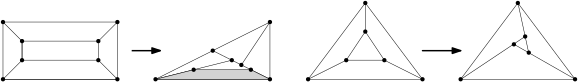
\includegraphics[width=0.9\textwidth]{sltr-example.png}
	\caption{Links einer der beiden drei-zusammenhängenden Graphen auf acht Knoten ohne SLTR und rechts ein Graph mit einer möglichen SLTR.}
\end{figure}

Um die Problemstellung greifbarer zu machen werden wir planare Graphen zusammen mit den drei Aufhängungen $a_1,a_2$ und $a_3$ als designierten Ecken einer möglichen SLTR betrachten. Einen Graphen zusammen mit einem äusseren Gebiet bzw. Aufhängungen zu betrachten, macht auch in sofern Sinn, dass kombinatorische Graphen existieren, von denen manche Einbettungen SLTRs zulassen, andere jedoch nicht, so wie in Abbildung \ref{10_example} zu sehen.

\begin{figure}
	\centering
  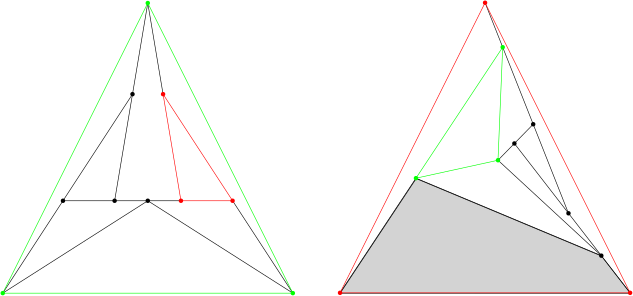
\includegraphics[scale=0.1]{10_example.png}
	\caption{Der kleinste drei-zusammenhängende Graph mit einer einer SLTR Einbettung und einer Auswahl der Aufhängung die kein SLTR zulässt.}
	\label{10_example}
\end{figure}

\begin{proposition}
Sei $G$ ein Graph mit Aufhängungen $a_1,a_2,a_3$ als äusseren Ecken einer SLTR. Weiter gebe es keinen Knoten von Grad zwei der in beiden angrenzenden Gebieten den Winkel $\pi$ hat\footnote{Ein solcher Knoten ist keine Aufhängung, da der Aussenwinkel grösser als $\pi$ ist. Alle anderen Knoten haben $\leq\pi$ Winkel. Somit können wir ihn durch eine gerade Kante zwischen seinen Nachbarn ersetzen und den resultierenden Graphen betrachten.}. Dann ist $G$ intern-drei-zusammenhängend\ref{int_3_con}.
\end{proposition}

%% TODO do i want the Proof??

Wir werden also von nun an, der Einfachheit halber intern-drei-zusammenhängende Graphen mit Aufhängungen betrachten, da alle anderen Graphen mit SLTR auf diese reduziert werden können. \\

Zu den Fragen, welche notwendigen und hinreichenden Bedingungen es für die Existenz von SLTRs gibt und  welche algorithmischen Ansätze es bei der Suche nach einer spezifischen Darstellung gibt haben Aerts und Felsner in \cite{af13}, \cite{af13h} und \cite{af15} schon einige Antworten geliefert, mit denen wir uns in den nächsten beidem Kapiteln beschäftigen werden. Zuerst müssen aber in diesem Kapitel noch ein paar notwendige Konzepte eingeführt werden.

\section{Schnyder Wälder}\label{sw}
Schnyder Wälder, im weiteren \textit{Schnyder Woods} wurden zuerst von Walter Schnyder zur Betrachung der Ordungs-Dimension planarer Graphen, als eine Färbung und Orientierung auf den inneren Kanten einer Triangulierung, betrachtet \cite{schnyder89}. In einem weiteren Resultat dienten sie zur Erlangung einer planaren Einbettung auf einem $n-2 \times n-2$ Netz\cite{schnyder90}. Im Folgenden werden wir die Verallgemeinerung auf drei-zusammenhängende plane Graphen durch Felsner \cite{felsner01} und die zu ihnen in Bijektion stehenden Schnyder Labelings einführen.\\
\begin{definition}[Schnyder Woods]
Ein Schnyder Wood ist eine Orientierung und Beschriftung der Kanten von $G$ mit den Labeln 1, 2 und 3 unter Berücksichtigung der folgenden Regeln\footnote{Alternativ kann hier auch anschaulicher einfach von rot, blau und grün gesprochen werden. Es wird davon ausgegangen, dass die Label zyklisch sortiert sind, sodass $i+1$ und $i-1$ immer definiert sind.}:
\begin{itemize}
\item[W1] Jede Kante ist entweder un- oder bigerichtet. Falls sie bigerichtet ist haben beide Richtungen unterschiedliche Label.
\item[W2] An jeder Aufhängung  $s_i$ exisitert eine nach ausssen gerichtete Kante ohne Endpunkt mit Label i.  
\item[W3] Jeder Knoten $v$ hat hat Ausgangsgrad eins zu jedem Label. Um $v$ existieren im Uhrzeigersinn eine Auskante mit Label 1, null oder mehr eingehende Kanten mit Label 3, eine Auskante mit Label 2, null oder mehr  eingehende Kanten mit Label 1, eine Auskante mit Label 2 und null oder mehr  eingehende Kanten mit Label 2.
\item[W4] Es existiert kein gerichteter Zykel mit einem Label.
\end{itemize}

\end{definition}

\begin{figure}[h]
	\centering
  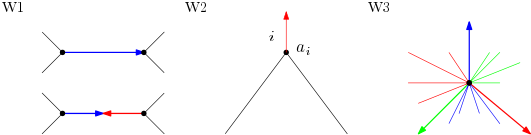
\includegraphics[width=0.9\textwidth]{schnyder_wood_def.png}
	\label{10_example}
\end{figure}

\begin{definition}[Schnyder Labeling]
Ein Schnyder Labeling ist eine Beschriftung Winkel von $G$ mit den Labeln 1, 2 und 3 unter Berücksichtigung der folgenden Regeln:
\begin{itemize}
\item[L1] Um jedes innere Gebiet bilden die Label im Uhrzeigersinn nichtleere Intervalle von 1en, 2en und 3en. Am äusseren Gebiet gilt dies gegen den Uhrzeigersinn.
\item[L2] An Aufhängung $a_i$ haben äusseren Winkel die Label i-1 und i+1 im Uhrzeigersinn mit der halben Auskante dazwischen und die inneren Winkel das Label i.\\
Um jeden inneren Knoten bilden die Label im Uhrzeigersinn nichtleere Intervalle von 1en, 2en und 3en.
\end{itemize} 

\end{definition}

\begin{theorem}
Schnyder Woods und Schnyder Labelings stehen in Bijektion zueinander.
// TODO  
\end{theorem}

// TODOBILD

\
\section{$\alpha$-Orientierungen}\label{alpha_orientations}

Für unseren Algorithmus in Kapitel \ref{main_algo} führen wir nun eine weitere zu Schnyder-Woods und Labelings in Bijektion stehende Struktur auf Graphen ein und halten uns dabei an \cite{felsner04}.

\begin{definition}[$\alpha$-Orientierung]
Sei $G=(V,E)$ ein ungerichteter Graph und $\alpha:V\mapsto\mathbb{N}$ eine Funktion auf $G$. Eine $\alpha$\textit{-Orientierung} ist eine Orientierung der Kanten von $G$, sodass der Ausgrad eines jeden Knoten $\alpha(v)$ entspricht. Somit muss gelten $$\text{outdeg}(v) = \alpha(v).$$
\end{definition}

Um von $\alpha$-Orientierungen zu Schnyder Woods zu gelangen müssen wir Primal-Dual Graphen betrachten die mit den nächsten beiden Definitionen eingeführt werden.

\begin{definition}[schwacher dualer Graph]
Sei $G$ ein planer Graph. $G^*$ der \textit{schwache duale Graph} von $G$. $G^*$ hat einen (Gebiets-)Knoten für jedes innere Gebiet von $G$. Für jede innerer Kante in $G$ fügen wir eine Kante zwischen den beiden (Gebiets-)Knoten $f,f'$ in $G^*$ ein, die adjazent zu dieser Kante in $G$ sind.
\end{definition}

\begin{definition}[Primal-Dual Graph]
Betrachte einen planen Graphen $G$ und seinen schwacher dualer Graphen $G^*$. Der \textit{Primal-Dual Graph} $G+G^*$ ist eine Vereinigung der Graphen $G$ und $G^*$ mit einem Knoten an jeder Kantenkreuzung. Die Menge der Knoten von $G+G^*$ besteht aus Knoten-Knoten, Kanten-Knoten und Gebiets-Knoten. Kanten in $G+G^*$ existieren, sowohl zwischen inzidenten Kanten und Knoten, als auch Kanten und Gebieten in $G$. Hinzu kommen Halbkanten\footnote{Kanten mit nur einem Randknoten die immer von diesem weg orientiert sind.} von den Kanten-Knoten und Knoten-Knoten am äusseren Gebiet von $G$.

Wenn wir einen Knoten $f_\infty$ für das äussere Gebiet hinzufügen und die Halbkanten zu diesem verlängern spricht man vom \textit{Abschluss} von $G+G^*$.

\end{definition}
Es ist leicht zu sehen, dass $G+G^*$ und sein Abschluss bipartit sind. Das folgende Theorem liefert eine Bijektion zwischen den Schnyder Woods auf $G$ und einer bestimmten $\alpha$-Orientierung auf dem Abschluss von $G+G^*$, die wir $\alpha_s$ nennen.

\begin{theorem}\label{alpha_bij}
Sei $G$ ein planer Graph mit Aufhängungen $\{a_1,a_2,a_3\}$, dann sind die folgenden Strukturen in Bijektion:
\begin{itemize}
\item [A1] Die Schnyder Woods auf $G$.
\item [A2] Die Schnyder Woods auf dem (schwachen) dualen Graphen $G^*$.
\item [A3] Die $\alpha_{s}$-Orientierungen des Abschlusses von $G+G^*$ mit $\alpha_s(v) = \alpha_s(f) = 3$ für jeden Knoten-Knoten $v$ und Gebiets-Knoten $f$,  $\alpha_s(e) = 1$ für jeden Kanten-Knoten $e$ und  $\alpha_s(f_\infty) = 0$.
\end{itemize}
\end{theorem}

\begin{remark}
Wir erhalten aus einem $\alpha_s$-Orientierung den Schnyder Wood, indem wir den drei Aufhängungen die Label rot, grün und blau geben und dann Schritt für Schritt die Kanten einfärben und dabei die Orientierung der Kanten aus $\alpha_s$ auf $G$ übernehmen. Wir erfüllen so bereits W1 und W2. Wenn nun an jedem Knoten an dem wir ankommen W3 bei der Einfärbung berücksichtigt wird erhalten wir einen eindeutigen Schnyder Wood auf $G$ (und somit auch auf $G^*$).
\end{remark}

\begin{figure}
	\centering
	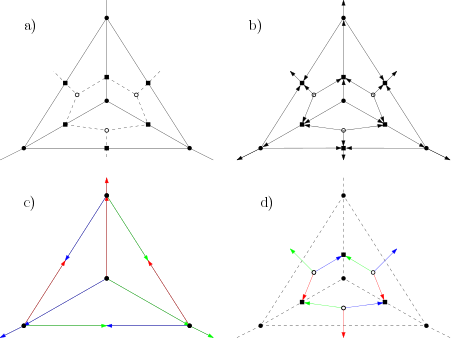
\includegraphics[width=0.7\textwidth]{alpha_ex2.png}
  \caption{ Der Primal-Duale Graph $K_4+K_4^*$ (a) mit einer $\alpha_s$-Orientiertung (b) und den zugehörigen Schnyder Woods auf $K_4$ (c) und $K^*_4$ (d). }
\end{figure}
\section{Flüsse auf Graphen}

Wir werden in Kapitel \ref{main_algo} einen gerichteten Graphen $\mathcal{N}$ konstruieren um auf diesem einen maximalen Fluss zu finden. Wir beschäftigen uns allgemein also mit der folgenden Problematik.

\begin{definition}[Gerichtetes-Multi-Fluss-Problem]\label{def_multi_flow}
Sei $D=(V,E)$ ein gerichteter Graph, im Weiteren auch Netzwerk genannt, mit den Kapaziäten $c:E\mapsto\mathbb{R}_{+}$, Paaren von ausgezeichneten Knoten $\{(s_1,t_1), ... ,(s_n,t_n)\}$ und positiven Bedarfen $\{d_1, ... ,d_n\}$, dann ist $\varphi=(\varphi_1, ... ,\varphi_n)$ ein zulässiger Fluss, falls
\begin{itemize}
\item[F1] $\forall (u,v) \in E : \sum_{i=1}^{n}{\varphi_i(u,v)} \leq c(u,v) $
\item[F2] $ \forall u \neq s_i,t_i : \sum_{w \in V} \varphi_i(u,w) - \sum_{w \in V} \varphi_i(w,u) $
\item[F3] $ \forall s_i : \sum_{w \in V} \varphi_i(s_i,w) - \sum_{w \in V} \varphi_i(w,s_i) = d_i $
\item[F4] $ \forall t_i : \sum_{w \in V} \varphi_i(w,s_i) - \sum_{w \in V} \varphi_i(s_i,w) = d_i $
\end{itemize}
\end{definition}

Wir wollen hier noch ein paar bekannte Resultate für den Fall $n=1$ festhalten, die wir später nutzen werden.

\begin{theorem}[Max-Flow Min-Cut]
$\varphi$ ist ein maximale Fluss in $\mathcal{N}$, genau dann, wenn für mindestens einen Schnitt $\mathcal{S} \subset E$ gilt $c(\mathcal{S}) = |\varphi|$. Die Kapazität eines minimalen Schnittes entspricht dem maximalen Fluss.
\end{theorem}

\begin{theorem}[Ganzzahliger Fluss]\label{theo_int_flow}
Sei $\mathcal{N}$ ein Netzwerk mit einer Quelle und einer Senke und alle Kapazitäten seien ganzzahlig, dann existiert auch ein maximaler Fluss $\varphi$, sodass der Fluss auf allen Kanten ganzzahlig ist. Es gilt also $|\varphi(e)| \in \mathcal{N}$ für alle $e\in E$.
\end{theorem}

\begin{remark}
Im Fall $n=1$ und Kapazitäten $c:E\mapsto\mathbb{N}$ impliziert die Existenz eines zulässigen Flusses also Existenz einer ganzzahligen Lösung, sowohl für gerichtete als auch ungerichtete Graphen, und diese lässt sich in polynomineller Zeit bestimmen. Für $n=2$ und ungerichtete Graphen gilt dies nach \cite{hu} ebenfalls. Für uns im Folgenden interessant wäre jedoch, wie wir sehen werden, der Fall $n=2$ für gerichtete Graphen. Leider ist hier im Allgemeinen die Lösung nur über Lineare Programmierung möglich und befindet sich somit in $\mathcal{NP}$.
\end{remark}
